\documentclass{beamer}

\providecommand{\rootdir}{../doc}

% \def\privateData{private_data}

% % % % % % % % % % % % % % % % % % % % % % % % % % % % % % % % % % % % % % % %

\usepackage[english]{babel}
\usepackage{ifthen}
\usepackage{color}
\usepackage{hhline}
\usepackage{adjustbox}
\usepackage{amsmath,amsfonts, amssymb}
\usepackage{mdframed}

\usepackage{tikz, skak}
\usetikzlibrary{fit, matrix, positioning, shapes, decorations.pathreplacing,
                shapes.geometric, chains, arrows, calc }




\newcommand{\red}[1]{{\color{red} #1}}
\newcommand{\green}[1]{{\color{green!50!black} #1}}
\newcommand{\orange}[1]{{\color{orange} #1}}
\newcommand{\blue}[1]{{\color{blue} #1}}


\newcommand{\resizeinput}[2][1]{%
  \resizebox{#1\textwidth}{!}{\input{#2}}%
}

% % % % % % % % % % % % % % % % % % % % % % % % % % % % % % % % % % % % % % % %
% from MathDefs.tex

\def\Re{\mathbb{R}}

\def\behaviour{\mathrm{behaviour}}
\def\act{\mathrm{act}}
\def\react{\mathrm{react}}
\def\state{\mathrm{state}}
\def\action{\mathrm{action}}
\def\msg{\mathrm{message}}

\def\coh{\mathrm{coh}}
\def\rel{\mathrm{rel}}
\def\fold{\mathit{fold}\,}

\def\Bool{\mathrm{Bool}}
\def\Candidate{\mathit{Candidate}}
\def\Details{\mathit{Details}}
% \def\Context{\mathit{Context}}


\providecommand{\letIn}[2]{
  \begin{aligned}[t]%
    & \mathit{let}\, #1 \\%
    & \mathit{in}~ #2%
  \end{aligned}%
}


% % % % % % % % % % % % % % % % % % % % % % % % % % % % % % % % % % % % % % % %

% https://tex.stackexchange.com/questions/45938/error-when-using-colour-in-author
\ifthenelse{\isundefined{\privateData}}
           {\author{\texorpdfstring{\color{red} Anonymous}{???}}}
           {\input{\privateData}}

% % % % % % % % % % % % % % % % % % % % % % % % % % % % % % % % % % % % % % % %

\title{University class schedule generation using personalizable agents negotiation}
\subtitle{Thesis for Master of Science in Intelligent Systems}
\institute[ITESM]{Tecnol\'{o}gico de Monterrey}
\logo{
\includegraphics{../doc/escudo-itesm}}
\date{May, 2017}

% % % % % % % % % % % % % % % % % % % % % % % % % % % % % % % % % % % % % % % %


\mode<presentation>

\begin{document}

\frame{\titlepage}

% % % % % % % % % % % % % % % % % % % % % % % % % % % % % % % % % % % % % % % %
% % % % % % % % % % % % % % % % % % % % % % % % % % % % % % % % % % % % % % % I
\section{University Class Scheduling Problem (UCSP)}
\subsection{The Problem}

\begin{frame}{University Class Scheduling Problem}
  \begin{block}{The Problem}
    \textbf{U}niversity \textbf{C}lass \textbf{S}cheduling \textbf{P}roblem (UCSP)
    consists in finding valid \alert{class} assignations for \underline{all} the
    participants:
    \begin{itemize}
      \item Groups / Students
      \item Professors
    \end{itemize}
  \end{block}
  \begin{block}{Class}
    A class is an educational event, that is formed with purpose of studying
    some \alert{discipline}.
    \begin{columns}
      \begin{column}{4cm}
        \\Takes place
        \begin{itemize}
          \item in a \underline{classroom}
          \item on given \underline{day}
          \item during given \underline{time}
        \end{itemize}
      \end{column}
      \begin{column}{3cm}
        Links together
        \begin{itemize}
          \item a \underline{group} and
          \item a \underline{professor}
        \end{itemize}
      \end{column}
    \end{columns}

  \end{block}
\end{frame}

\begin{frame}
  \begin{columns}
    \begin{column}{4cm}
      \begin{block}{Schedule}
        The complete schedule consists of all the classes of all the participants,
        that can be seen as points in 5-dimensional space. It can be decomposed
        into a set of \alert{timetables}.
      \end{block}
    \end{column}
    \begin{column}{7cm}
        \resizeinput{\rootdir/img/ScheduleHypercube/GRPT-content.tikz}
    \end{column}
  \end{columns}
\end{frame}

\begin{frame}
  \begin{block}{Timetable}
    Timetable is projection of the schedule on the person/entity.
    It is a 2-dimensional table, that contains \underline{only} the classes
    of projection target.
  \end{block}
  \begin{columns}
    \begin{column}{.5\textwidth}
      \centering
      \begin{tabular}{|c||c|c|c|}
  \hline & Mon & Tue & $\cdots$ \\
  \hhline{|=#=|=|=|}
  08:30 -- 08:40 & x & & \\\hline
  08:40 -- 08:50 & x & & \\\hline
  08:50 -- 09:00 & x & & \\\hline
  $\vdots$\quad~--~\quad$\vdots$ & & & \\\hline
  09:50 -- 10:00 & x & & \\\hline
  10:00 -- 10:10 &   & & \\\hline
  10:10 -- 10:20 & y & & \\\hline
  10:20 -- 10:30 & y & & \\\hline
  $\vdots$\quad~--~\quad$\vdots$ & & & \\\hline
\end{tabular}

    \end{column}
    \begin{column}{.5\textwidth}
      \centering
      \begin{tabular}{|c||c|c|c|}
  \hline & Mon & Tue & $\cdots$ \\
  \hhline{|=#=|=|=|}
  08:30 -- 09:15 & x & & \\\hline
  09:25 -- 10:10 & x & & \\\hline
  10:30 -- 11:15 & y & & \\\hline
  11:25 -- 12:10 & y & & \\\hline
  Lunch          &   & & \\\hline
  13:25 -- 14:10 & z & & \\\hline
  14:20 -- 15:05 & z & & \\\hline
  15:25 -- 16:10 &   & & \\\hline
  $\vdots$\quad~--~\quad$\vdots$ & & & \\\hline
\end{tabular}

    \end{column}
  \end{columns}
  % \centering
  % \begin{tabular}{|c||c|c|c|c|c|c|}
  \hline & Mon & Tue & Wed & Thu & Fri & Sat \\
  \hhline{|=#=|=|=|=|=|=|}
  08:00 -- 08:30 & x & & & w & & \\\hline
  08:30 -- 09:00 & x & & & w & & \\\hline
  09:00 -- 09:30 & x & & & z & & \\\hline
  09:30 -- 10:00 & y & & & z & & \\\hline
  10:00 -- 10:30 & y & & & z & & \\\hline
  $\vdots$\quad~--~\quad$\vdots$ & & & & & & \\\hline
  21:00 -- 21:30 &   & & & & & \\\hline
  21:30 -- 22:00 &   & & & & & \\\hline
\end{tabular}

\end{frame}

% % % % % % % % % % % % % % % % % % % %
\subsection{Constraints}

\begin{frame}[label=constraints]{University Class Scheduling Constraints}
  \fbox{
    \begin{columns}[t]
      ~~Independent
      \begin{column}{.4\textwidth}
        \begin{block}{Class}
          \begin{itemize}
            \item Group needs
            \item Professor can teach
            \item Classroom is suitable
          \end{itemize}
        \end{block}
      \end{column}
      \begin{column}{.4\textwidth}
        \begin{block}{Time}
          \begin{itemize}
            \item Classes non intersection
          \end{itemize}
        \end{block}
      \end{column}
    \end{columns}
  }
  \\[.7cm]
  \fbox{
    \begin{columns}[t]
      Personal
      \begin{column}{.4\textwidth}
        \begin{block}{Obligations}
          \begin{itemize}
            \item Personal \alert{strong} restrictions
          \end{itemize}
        \end{block}
      \end{column}
      \begin{column}{.4\textwidth}
        \begin{block}{Preferences}
          \begin{itemize}
            \item Personal \alert{weak} restrictions
          \end{itemize}
        \end{block}
      \end{column}
    \end{columns}
  }
\end{frame}

\begin{frame}{Class Constraints}
  \centering
  \resizeinput[.5]{\rootdir/img/Capabilities.tikz}
\end{frame}

% % % % % % % % % % % % % % % % % % % % % % % % % % % % % % % % % % % % % % % III
\section{Formal Definition}

\begin{frame}{University Class Scheduling Problem}
  \centering
  \begin{block}{Required Data}
    \begin{columns}[t]
      \begin{column}{.4\textwidth}
        \begin{block}{Disciplines $\{d_i\}$}
          \begin{itemize}
            \item academic program
            \item special requirements
          \end{itemize}
        \end{block}
      \end{column}
      \begin{column}{.4\textwidth}
        \begin{block}{Groups $\{g_i\}$}
          \begin{itemize}
            \item disciplines needed
            \item personal constraints
          \end{itemize}
        \end{block}
      \end{column}
    \end{columns}
    \begin{columns}[t]
      \begin{column}{.4\textwidth}
        \begin{block}{Classrooms $\{r_i\}$}
          \begin{itemize}
            \item capacity
            \item equipment
          \end{itemize}
        \end{block}
      \end{column}
      \begin{column}{.4\textwidth}
        \begin{block}{Professors $\{p_i\}$}
          \begin{itemize}
            \item able to teach (disciplines)
            \item personal constraints
          \end{itemize}
        \end{block}
      \end{column}
    \end{columns}
    \begin{columns}
      \begin{column}{.4\textwidth}
        \begin{block}{Working Days $\{\bar{d}_i\}$}\end{block}
      \end{column}
      \begin{column}{.4\textwidth}
        \begin{block}{Discrete Time $\{\bar{t}_i\}$}\end{block}
      \end{column}
    \end{columns}
  \end{block}
\end{frame}

\begin{frame}{University Class Scheduling Problem}
  \begin{block}{Class Core $\mathrm{cc} \sim \left< d, g, p \right>$}
    \emph{possible} class (of discipline $d$) for group $g$,
    taught by professor $p$
  \end{block}
  \begin{block}{Class $ c \sim \left< \mathrm{cc}, r, \bar d, \bar t_b, \bar t_e \right> $}
    \emph{concrete} class, with day, time (beginning \& end) and room
  \end{block}
  \begin{block}{Candidate $\tilde{c}_a=\{c ~|~ c\,\mathrm{mensions}\,a\}$}
    set of \alert{valid} classes, assessed using \underline{coherence},
    proposed by $a$
  \end{block}
  \begin{block}{Schedule $= \bigcup\limits_{\forall\,a}\tilde{c}_a$}
    set of \alert{\underline{all}} proposed classes, assessed by every group and
    professor

  \end{block}
\end{frame}

\frame{
  \trimbox{30pt 0 0 0}{
    \resizeinput{\rootdir/img/ConnectionMatrix/Candidates-content.tikz}
  }
}

% % % % % % % % % % % % % % % % % % % % % % % % % % % % % % % % % % % % % % IV
\section{Coherence}

\begin{frame}
  \begin{block}{Coherence}
    In simple worlds, \emph{coherence} is a state or measure of some \emph{pieces}
    fitting together into a whole. Coherence can be applied to almost any aspect of
    the universe.
  \end{block}
  \begin{quote}
    The consistency or \emph{coherence} within a logical or mathematical
    system, means that $p$ and $\neg p$ must not be derivable from the
    basic assumptions in accordance with the observance of the syntactical
    rules (Daya, 1960).
  \end{quote}
  \begin{quote}
    Coherence theory is a psychologically motivated motivational cognitive theory with
    foundations in philosophy that approaches problems in terms of the satisfaction
    of multiple constraints within networks of highly interconnected elements
    (Sindhu, 2010).
  \end{quote}
\end{frame}


\begin{frame}{Coherence}
  \begin{block}{Coherence by Thagard}
    Thagard (1998) claimed that \alert{coherence} can be understood in terms of
    \alert{maximal satisfaction of multiple constraints}.

    \medskip
    By Thagard, coherence problem is about \underline{partitioning a graph} of
    \emph{information pieces}, interconnected by positive or negative weighted
    constraints, that enhance or diminish partition's coherence.
  \end{block}
\end{frame}
\begin{frame}{Coherence}
  \begin{block}{Information Graph Splitting}
    The information graph $\mathcal{V}$ consists of
    classes $C_1,\dots,C_4$, also there are three possibilities for
    class $C_1$ placement and two for class $C_4$.\\\bigskip
    \begin{columns}
      \begin{column}{.3\textwidth}
        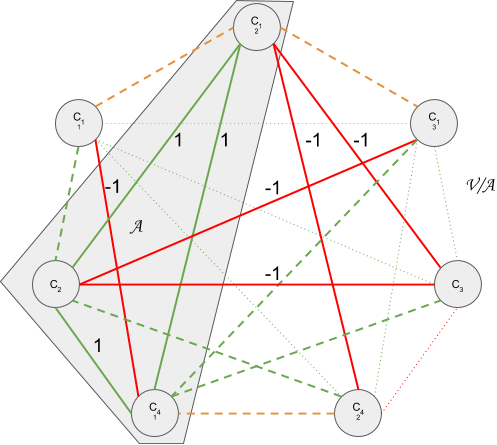
\includegraphics[width=\textwidth, trim={20pt 20pt 100pt 20pt}]
                        {\rootdir/img/UAB-splitting.png}
      \end{column}
      \begin{column}{.8\textwidth}
        \qquad\quad A relation is
        \begin{mdframed}[leftmargin=2cm, hidealllines=true]
          \begin{itemize}
            \item[\red{\emph{inconsistent}}], if two classes intersect in time;
            \item[\yellow{\emph{same class}}], if two classes differ only by time;
            \item[\green{\emph{consistent}}], otherwise.
          \end{itemize}
        \end{mdframed}
      \end{column}
    \end{columns}
  \end{block}
\end{frame}

% % % % % % % % % % % % % % % % % % % %
\subsection{Contexts}

\begin{frame}{Coherence}
  \begin{block}{Contexts}
    Describe aspects of coherence problem.
    \begin{columns}[t]
      \begin{column}{.5\textwidth}
        \begin{block}{Original}
          Proposed by Sindhu (2010) \\\medskip
          \begin{itemize}
            \item Contexts represent BDI
            \item Each context has own logic
            \item Contexts are connected by
                  \emph{bridge rules}
          \end{itemize}
        \end{block}
      \end{column}
      \begin{column}{.5\textwidth}
        \begin{block}{Proposed}
          \begin{itemize}
            \item Contexts represent groups of constraints
            \item \underline{Assess coherence}
                  of the given information and tell whether
                  it is \underline{coherent}
            \item Candidate is \alert{\underline{propagated}} through
                  the contexts
          \end{itemize}
        \end{block}
      \end{column}
    \end{columns}
  \end{block}
\end{frame}

\againframe{constraints}

\begin{frame}{Contexts}
  \begin{columns}
    \begin{column}{.2\textwidth}\end{column}
    \begin{column}{.2\textwidth}
      \tikz\draw[->, >=stealth, double, thick]
                (0,0)  node[yshift=10pt] {Candidate $\tilde{c}$}
                  --
                (0,-5) node[yshift=-10pt] {Assessed candidate $\tilde{c}$};
    \end{column}
    \begin{column}{.5\textwidth}
      \vfill
      \begin{enumerate}
        \item Common / Independent
          \begin{enumerate}
            \item Class constraints
            \item Time constraints
          \end{enumerate}
        \item Internal / Personal
          \begin{enumerate}
            \item Obligations (strong)
            \item Preferences (weak)
          \end{enumerate}
        \item \underline{External}\\
              communicates, works towards
              \emph{common goal}
      \end{enumerate}
      \vfill
    \end{column}
    \begin{column}{.3\textwidth}\end{column}
  \end{columns}
\end{frame}

% % % % % % % % % % % % % % % % % % % % % % % % % % % % % % % % % % % % % % % III
\section{Formal Definition}

\begin{frame}{University Class Scheduling Problem}
  \centering
  \begin{block}{Required Data}
    \begin{columns}[t]
      \begin{column}{.4\textwidth}
        \begin{block}{Disciplines $\{d_i\}$}
          \begin{itemize}
            \item academic program
            \item equipment requirements
          \end{itemize}
        \end{block}
      \end{column}
      \begin{column}{.4\textwidth}
        \begin{block}{Groups $\{g_i\}$}
          \begin{itemize}
            \item disciplines needed
            \item personal constraints
          \end{itemize}
        \end{block}
      \end{column}
    \end{columns}
    \begin{columns}[t]
      \begin{column}{.4\textwidth}
        \begin{block}{Classrooms $\{r_i\}$}
          \begin{itemize}
            \item capacity
            \item equipment
          \end{itemize}
        \end{block}
      \end{column}
      \begin{column}{.4\textwidth}
        \begin{block}{Professors $\{p_i\}$}
          \begin{itemize}
            \item able to teach (disciplines)
            \item personal constraints
          \end{itemize}
        \end{block}
      \end{column}
    \end{columns}
    \begin{columns}
      \begin{column}{.4\textwidth}
        \begin{block}{Working Days $\{\bar{d}_i\}$}\end{block}
      \end{column}
      \begin{column}{.4\textwidth}
        \begin{block}{Discrete Time $\{\bar{t}_i\}$}\end{block}
      \end{column}
    \end{columns}
  \end{block}
\end{frame}

\begin{frame}{University Class Scheduling Problem}
  \begin{block}{Class Core $\mathrm{cc} \sim \left< d, g, p \right>$}
    \emph{possible} class (of discipline $d$) for group $g$,
    taught by professor $p$
  \end{block}
  \begin{block}{Class $ c \sim \left< \mathrm{cc}, r, \bar d, \bar t_b, \bar t_e \right> $}
    \emph{concrete} class, with day, time (beginning \& end) and room
  \end{block}
  \begin{block}{Candidate $\tilde{c}_a=\{c ~|~ c\,\mathrm{mensions}\,a\}$}
    set of \alert{valid} classes, assessed using \underline{coherence},
    proposed by $a$
  \end{block}
  \begin{block}{Schedule $= \bigcup\limits_{\forall\,a}\tilde{c}_a$}
    set of \alert{\underline{all}} proposed classes, assessed by every group and
    professor

  \end{block}
\end{frame}

\frame{
  \trimbox{30pt 0 0 0}{
    \resizeinput{\rootdir/img/ConnectionMatrix/Candidates-content.tikz}
  }
}

% % % % % % % % % % % % % % % % % % % % % % % % % % % % % % % % % % % % % % % IV
\section{Coherence}

\begin{frame}
  \begin{block}{Coherence}
    In simple worlds, \emph{coherence} is a state or measure of some \emph{pieces}
    fitting together into a whole. Coherence can be applied to almost any aspect of
    the universe.
  \end{block}
  \begin{quote}
    The consistency or \emph{coherence} within a logical or mathematical
    system, means that $p$ and $\neg p$ must not be derivable from the
    basic assumptions in accordance with the observance of the syntactical
    rules (Daya, 1960).
  \end{quote}
  \begin{quote}
    Coherence theory is a psychologically motivated motivational cognitive theory with
    foundations in philosophy that approaches problems in terms of the satisfaction
    of multiple constraints within networks of highly interconnected elements
    (Sindhu, 2010).
  \end{quote}
\end{frame}


\begin{frame}{Coherence}
  \begin{block}{Coherence by Thagard}
    Thagard (1998) claimed that \alert{coherence} can be understood in terms of
    \alert{maximal satisfaction of multiple constraints}.

    \medskip
    By Thagard, coherence problem is about \underline{partitioning a graph} of
    \emph{information pieces}, interconnected by positive or negative weighted
    constraints, that enhance or diminish partition's coherence.
  \end{block}
\end{frame}
\begin{frame}{Coherence}
  \begin{block}{Information Graph Splitting}
    The information graph $\mathcal{V}$ consists of
    classes $C_1,\dots,C_4$, also there are three possibilities for
    class $C_1$ placement and two for class $C_4$.\\\bigskip
    \begin{columns}
      \begin{column}{.3\textwidth}
        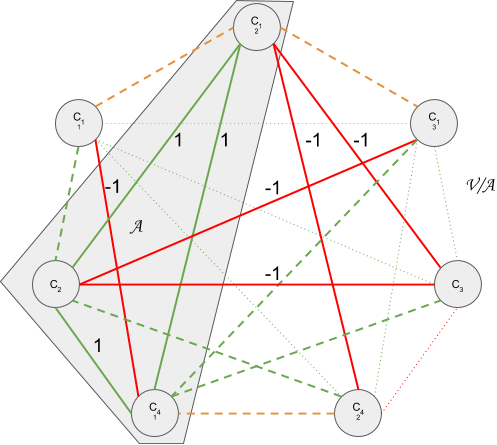
\includegraphics[width=\textwidth, trim={20pt 20pt 100pt 20pt}]
                        {\rootdir/img/UAB-splitting.png}
      \end{column}
      \begin{column}{.8\textwidth}
        \qquad\quad A relation is
        \begin{mdframed}[leftmargin=2cm, hidealllines=true]
          \begin{itemize}
            \item[\red{\emph{inconsistent}}], if two classes intersect in time;
            \item[\orange{\emph{same class}}], if two classes differ only by time;
            \item[\green{\emph{consistent}}], otherwise.
          \end{itemize}
        \end{mdframed}
      \end{column}
    \end{columns}
  \end{block}
\end{frame}

% % % % % % % % % % % % % % % % % % % %
\subsection{Contexts}

\begin{frame}{Coherence}
  \begin{block}{Contexts}
    Describe aspects of coherence problem.
    \begin{columns}[t]
      \begin{column}{.5\textwidth}
        \begin{block}{Original}
          Proposed by Sindhu (2010) \\\medskip
          \begin{itemize}
            \item Contexts represent BDI
            \item Each context has own logic
            \item Contexts are connected by
                  \emph{bridge rules}
          \end{itemize}
        \end{block}
      \end{column}
      \begin{column}{.5\textwidth}
        \begin{block}{Proposed}
          \begin{itemize}
            \item Contexts represent groups of constraints
            \item \underline{Assess coherence}
                  of the given information and tell whether
                  it is \underline{coherent}
            \item Candidate is \alert{\underline{propagated}} through
                  the contexts
          \end{itemize}
        \end{block}
      \end{column}
    \end{columns}
  \end{block}
\end{frame}





\begin{frame}{Context}
  % Context represents an aspect for optimization/restriction (group of constraints).
  \begin{block}{Defines}
    \begin{enumerate}
      \item Context-specific information
      \item \underline{Relations} over the information graph $\{\rel\}$
      \item \underline{Relations combination} associative function $f^\cup$
      \item Context-specific \emph{Details}
      \item Context-specific threshold $\Theta$
    \end{enumerate}
  \end{block}
  \begin{block}{Assessment Modes}
    \begin{itemize}
      \item Preliminary
      \item Final
    \end{itemize}
  \end{block}
\end{frame}

\begin{frame}{Context: Relations}
  \begin{block}{Relations}
    \begin{itemize}
      \item Over whole graph
        \begin{align*}
          & \rel: \lbrace I \rbrace \mapsto \Re \times \Details \\
          & \coh[\rel](\tilde{c}) = rel(\tilde{c})
        \end{align*}
      \item Binary
        \begin{align*}
          & \rel: I \times I \mapsto \Re \times \Details \\
          & f^\cup_2: (\Re \times \Details) \times
                      (\Re \times \Details)
               \mapsto \Re \times \Details \\[0.3em]
          & \coh[\rel](\tilde{c}) = \fold (f^\cup_2[\rel]) ~
              \left(\lbrace \rel(c_a,c_b) ~|~ \forall\, c_a,c_b \in \tilde{c}
                                      , ~ a \not= b \rbrace\right)
        \end{align*}
    \end{itemize}
  \end{block}
\end{frame}

\begin{frame}{Context: Assessment}
  \begin{block}{Relations Combination}
    \begin{align*}
      & f^\cup: (\Re \times \Details) \times
                (\Re \times \Details)
         \mapsto \Re \times \Details \\
      & \mathrm{assess}[\mathrm{context}]: \Candidate \mapsto
                                           \Re \times \Details
      \\[0.3em]
      & \mathrm{assess}[\mathrm{context}](\tilde{c}) =
        \fold (f^\cup) ~ \left(
        \lbrace \coh[\rel](\tilde{c}) ~|~
                \forall\, \rel \in \mathrm{rels}(\mathrm{context})
        \rbrace\right)
    \end{align*}
  \end{block}
  \begin{block}{Coherence Assessment at Context}
    \begin{align*}
      & \coh[\mathrm{context}]: \Candidate \mapsto \Re \times
                                \Bool \times \Details
      \\[0.3em]
      & \coh[\mathrm{context}](\tilde{c}) =
          \letIn{ \left<x,d\right> = \mathrm{assess}[\mathrm{context}](\tilde{c}) }
                {\left<x, x \geq \Theta, d\right>}
    \end{align*}
  \end{block}
\end{frame}


% % % % % % % % % % % % % % % % % % % %

\againframe{constraints}

\begin{frame}{Contexts}
  \begin{columns}
    \begin{column}{.2\textwidth}\end{column}
    \begin{column}{.2\textwidth}
      \tikz\draw[->, >=stealth, double, thick]
                (0,0)  node[yshift=10pt] {Candidate $\tilde{c}$}
                  --
                (0,-5) node[yshift=-10pt] {Assessed candidate $\tilde{c}$};
    \end{column}
    \begin{column}{.7\textwidth}
      \vfill
      \begin{enumerate}
        \item Common / Independent
          \begin{enumerate}
            \item Class constraints: \textit{true}/\textit{false}
            \item Time constraints: \textit{true}/\textit{false}
          \end{enumerate}
        \item Internal / Personal
          \begin{enumerate}
            \item Obligations (strong): \textit{true}/\textit{false}
            \item Preferences (weak):   $(0,1]$
          \end{enumerate}
        \item \underline{External}: $[0,1]$\\
              communicates,\\
              works towards \emph{common goal}
      \end{enumerate}
      \vfill
    \end{column}
    \begin{column}{.3\textwidth}\end{column}
  \end{columns}
\end{frame}

% % % % % % % % % % % % % % % % % % % % % % % % % % % % % % % % % % % % % % % V
\section{Agents}

\begin{frame}{Agents}
  The notion of agent appears in Aristotle's works
   \begin{quote}
     Entity that acts with a purpose, within a social context.
   \end{quote}\\\medskip
  The prætorian roman law defined an agent as
    \begin{quote}
      A person who acts on behalf of a principal for
      a specific purpose and under limited delegation of authority and
      responsibility.
    \end{quote}\\\medskip
  The earliest use of the term agent in AI was
    \begin{quote}
      A program that is capable of executing an action vicariously.
    \end{quote}
\end{frame}

% ?? Solve CSPs with Agents ??

\begin{frame}
  \centering
  \begin{block}{An Agent}
    is \emph{computer system}, that
    \begin{enumerate}
      \item has a degree of autonomy in determining its behavior,
      \item interacts with humans and or other agents,
      \item perceives the environment and reacts to it, and
      \item exhibits a goal directed behavior.
    \end{enumerate}
  \end{block}
  \begin{block}{A Negotiation}
     is a process of \underline{communication} between heterogeneous agents
     with goal of resolving some common problem.
  \end{block}
  \begin{block}{A Negotiating Agent}
     is an \emph{isolated} \emph{proactive} computational entity,
     capable of sending and receiving messages.
  \end{block}
\end{frame}

\begin{frame}{Agents}
  \begin{block}{Behaviour}
    An agent is defined by it's behaviour:
    \begin{align*}
      \behaviour_\act   &: \state \mapsto \action \\
      \behaviour_\react &: \state \times \msg \mapsto \action
    \end{align*}
    % The agents must use a common \emph{communication protocol}, to ensure
    % understanding between agents of the same or different roles.
  \end{block}
  \begin{block}{Role}
    A role describes whom or what an agents represents in the negotiation and
    defines \emph{behaviour archetype}.
  \end{block}
  \begin{block}{Implementation}
    Agents are implemented in \underline{Haskell} using
    \emph{Software Transactional Memory} (STM)
    --- a promising concurrency paradigm.
  \end{block}
\end{frame}

% % % % % % % % % % % % % % % % % % % % % % % % % % % % % % % % % % % % % % % %




% % % % % % % % % % % % % % % % % % % % % % % % % % % % % % % % % % % % % % VI
\section{Agent Roles}

\begin{frame}{Agent Roles}

  \begin{center}
  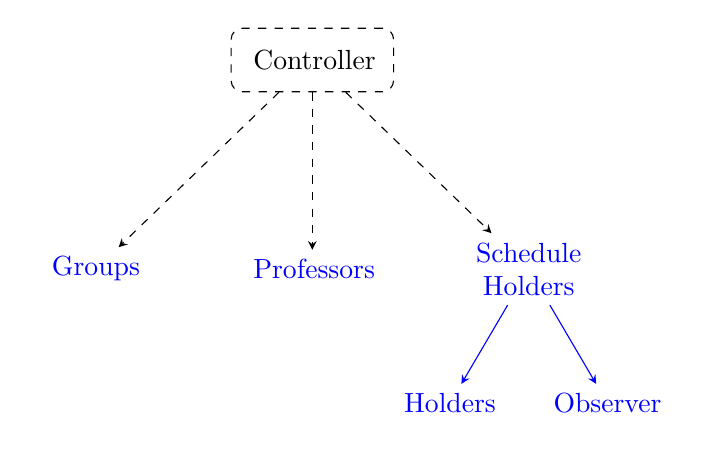
\begin{tikzpicture}[every node/.style={text width=1.5cm, align=center}]
    \node[draw, rounded corners,dashed, inner sep=8pt] (C) {Controller};
    \node[color=blue, below=2cm of C] (P) {Professors};
    \node[color=blue, left=of P]  (G) {Groups};
    \node[color=blue, right=of P] (H) {Schedule Holders};
    \draw[->, >=stealth, dashed] (C) -- (G);
    \draw[->, >=stealth, dashed] (C) -- (P);
    \draw[->, >=stealth, dashed] (C) -- (H);
    \node[color=blue, below=of H, xshift=-1cm] (HH) {Holders};
    \node[color=blue, below=of H, xshift=1cm]  (HO) {Observer};
    \draw[->, >=stealth, blue] (H) -- (HH);
    \draw[->, >=stealth, blue] (H) -- (HO);
  \end{tikzpicture}
  \end{center}

  \bigskip

  \blue{Groups} and \blue{Observer} have \underline{active} behaviour, while \\
  \blue{Professors} and \blue{Holders} exhibit only the \underline{reactive} one.

\end{frame}

% % % % % % % % % % % % % % % % % % % %
\subsection{Group}


% % % % % % % % % % % % % % % % % % % % Candidates Creation

% \againframe{candidate-def}  !!!!!!!!!!!!!!!!!!!!!!!!!!!!!!!!!!!!!!!!!!!!!!!!!!!!!!!!!!!!!!!!!!!!!!!!!!!!!!!!!!!!!!!!!!!!!!!!!!!!!!!!!!!!!!!!!!!!!!!!!!!!!!!!!!

\begin{frame}{Group: Candidates Creation}
  \centering
  Each class consists of \emph{class-core} and \emph{instance} assignations

  \bigskip \bigskip

  \begin{block}{Class-Cores Pool}
    is a lazy random sequence of class-cores,
    that contain \underline{a class for each discipline}, needed by the group.

    \medskip

    \begin{enumerate}
      \item For each discipline needed select professors, that can teach it.
            Randomize professors lists.
      \item Lazily generate all possible combinations \emph{professor} -- \emph{discipline}.
      \item When getting next combination, assign the generating \emph{group}.
    \end{enumerate}
  \end{block}
\end{frame}

\begin{frame}{Group: Candidates Creation}
  \begin{block}{Day -- Time -- Room}
    \begin{enumerate}
      \item Generate random \emph{day}.
      \item Select random \emph{classroom}.
      \item Generate \emph{beginning time}.
      \item Get class duration from the \emph{discipline}, contained in argument class-core.
            Calculate \emph{end time}.
      \item Test \emph{end time} consistency (upper bound).
      \item Test \emph{time consistency} of the values from (1-4) using the history.
      \item If new values are consistent, add them to history, assign to class-core
            and return it.
            Otherwise, repeat from (1).
    \end{enumerate}
    Assignation for classes of same possible candidate is done with same
      history.
  \end{block}
\end{frame}


% % % % % % % % % % % % % % % % % % % % Action Part I

\begin{frame}{Group Action}
  \marginbox{-30pt 0 0 0}{
    \clipbox{-65pt 350 20 0}{ %{left bottom right top}
      \resizebox{\textwidth}{!}{
        \colorlet{darkgreen}{green!50!black}

\begin{tikzpicture}[trim left, trim right=15.5cm,
  start chain=0 going below,
  gact/.style={on chain=0, text width=5cm, minimum height=30pt, align=center},
  start chain=1 going below,
  amsg/.style={on chain=1, text width=4.5cm, minimum height=30pt},
  start chain=2 going below,
  hmsg/.style={on chain=2, text width=4.5cm, minimum height=30pt},
  hact/.style={text width=4.5cm, minimum height=30pt, align=center},
  ifshape/.style={draw, diamond, shape aspect=3, text width=3cm},
  gact_if/.style={gact, ifshape},
  extracol/.style={text width=4.5cm},
  % mymark/.style={draw, circle, double, thick, inner sep=2pt},
  % goto/.style={draw, circle, double, dotted, inner sep=2pt},
  arr/.style={->, >=stealth},
  flow/.style={arr, double, line width=2pt},
  flow2/.style={flow, triangle 90 cap->, shorten <=-5pt},
  msg/.style={arr, sloped, rounded corners},
  center/.style={align=center}
  ]

% % % % % % % % % % % % % % % % % % % % % % % % % % % % % % % % % % % % % % % %
% Group ACT
\begin{scope}

\node[gact, draw, double] (G-Act-label) {\textbf{Group Action}};


\def\rshift{15pt}
\node[gact, draw] (G-create-c) {Create candidate $\tilde{c}=\{c\}$ --- set of classes};
% \node[mymark, left=20pt of G-create-c, yshift=30pt] (mark-Beta) {\Large $\beta$};
\node[right=of G-create-c, yshift=\rshift, draw, extracol] (G-create-cc)
    {Get \emph{class core} from \emph{pool}};
\node[right=of G-create-c, yshift=-\rshift, draw, extracol] (G-create-DTR)
    {Assign \emph{day}, \emph{time} and \emph{room}};
\draw (G-create-c) -- (G-create-cc);
\draw (G-create-c) -- (G-create-DTR);


\def\rshift{20pt}
\node[gact, draw, yshift=-20pt] (G-assess) {Assess coherence of $\tilde{c}$};
\node[right=of G-assess, yshift=\rshift, draw, extracol] (G-assess-i)
    {Internal: obligation \& preferences};
\node[right=of G-assess, yshift=-\rshift, draw, extracol] (G-assess-e)
    {External: neighbors' opinions combination };
\draw (G-assess) -- (G-assess-i);
\draw (G-assess) -- (G-assess-e);


\node[gact_if] (G-coherent) {Is \underline{coherent}?};
\node[right=33pt of G-coherent, extracol, draw, align=center] (G-put-c)
    {Put candidate $\tilde{c}$ into the \emph{common solution}};

\def\rshift{1.5cm}
\node[gact, draw, ellipse, text width=2cm] (G-put-resp) {\textit{Response}};
\node[right=1cm of G-put-resp.east, inner sep=0pt] (G-put-resp-right) {};
\node[below=of G-put-resp, xshift=-\rshift] (G-put-succ) {\underline{Success}};
\node[below=of G-put-resp, xshift=\rshift, text width=4cm, align=center] (G-put-fail)
    {\underline{Conflict} with candidates $\{\tilde{c}_j\}$};


\node[below=20pt of G-put-succ, draw, double, color=darkgreen] (G-sleep) {\Large \textbf{Sleep}};


\def\rshift{1.5cm}
\node[gact, yshift=-2.5cm, draw] (G-prove)
    {Try to \underline{prove} that candidate $\tilde{c}$ is \emph{better}
      than \underline{any} conflicting candidate $\tilde{c}_j$, by comparing:
      % or \underline{yield}.
      };

\begin{scope}[every node/.style={minimum height=30pt, align=center}] % , draw, dashed
  \node[below=of G-prove, xshift=-\rshift, text width=2cm] (G-prove-rare)
      {Candidate's \underline{``rareness''}};
  \node[below=of G-prove, xshift=\rshift, yshift=18pt, inner sep = 1pt,
        draw, circle, text width=2cm, dashed] (G-prove-deep)
      {\underline{Deep} external coherence};
\end{scope}
\path[] (G-prove-rare) -- node []{\Huge $>$} (G-prove-deep);


\node[gact_if, yshift=-2cm, shape aspect=2, inner sep = 0pt] (G-prove-res)
    {Could beat \underline{all} conflicting candidates?};
% \node[goto, left=5pt of G-prove-res, yshift=1cm] (G-goto-Beta-1) {\Large $\beta$};
\node[right=of G-prove-res, extracol, draw, align=center] (G-demand-placement)
    {\underline{Demand} placement of $\tilde{c}$, \\
      providing \emph{superiority proofs}};


% % % % % % % % % % % % % % % %

\draw[flow] (G-Act-label) -- (G-create-c);
\draw[flow] (G-create-c) -- (G-assess);
\draw[flow] (G-assess) -- (G-coherent);

% \draw[flow] (mark-Beta) -- ($(G-create-c.west) + (0,2pt)$);

\draw[flow2] (G-coherent.west) node[below, xshift=-10pt] {\large \textbf{No}}
             -- ++(-20pt,0) |- ($(G-create-c.west) - (0,7pt)$);
\draw[flow2] (G-coherent) -- node[below, xshift=-5pt] {\large \textbf{Yes}}
             (G-put-c);

\draw[flow2] (G-put-resp-right) -- (G-put-resp);
\draw[flow] (G-put-resp) -- (G-put-succ);
\draw[flow] (G-put-resp) -- (G-put-fail);

\draw[flow, shorten <=-3pt] (G-put-succ) -- (G-sleep);
\draw[flow, shorten <=-3pt] (G-put-fail) -- (G-prove.north-|G-put-fail);

\draw[flow] (G-prove) -- (G-prove-rare);
\draw[flow] (G-prove) -- (G-prove-deep);

\draw[flow, dashed] (G-prove-rare) -- (G-prove-res);
\draw[flow, dashed] (G-prove-deep) -- (G-prove-res);

\draw[flow2] (G-prove-res.west) node[below, xshift=-8pt] {\large \textbf{No}}
             -- ++(-25pt,0) |- ($(G-create-c.west) + (0,7pt)$);
            %  (G-goto-Beta-1);
\draw[flow2] (G-prove-res) -- node[below, xshift=-5pt] {\large \textbf{Yes}}
             (G-demand-placement);
\end{scope}

% % % % % % % % % % % % % % % % % % % % % % % % % % % % % % % % % % % % % % % %
% Professor / Group MSG
\begin{scope}

\node[amsg, right=7cm of G-Act-label, draw, double, center] (A-Msg-label)
    {\textbf{Professor / Group \\ Messages} (of agent $a_k$)};

\node[amsg, draw] (A-opinion) % , right=2cm of G-assess-i
    {\underline{\textbf{Opinion}} about candidate $\tilde{c_i}$ of group $g_i$
      by agent $a_k$ is agent's \emph{internal coherence} of the candidate.};

\draw[msg] ($(G-assess-e.east) + (0, 4pt)$)
           node[right, yshift=20pt, text width=2.2cm, center, xshift=7pt]
                {\underline{ask opinion} \\ of $p_k$ about $\tilde{c}$}
           -| ($(A-opinion.south) - (1cm, 0)$);
\draw[msg] ($(A-opinion.south) + (1cm, 0)$)
           node[rotate=90, above, xshift=-1cm] {\emph{opinion}}
           |- ($(G-assess-e.east) - (0, 4pt)$);

% % % % % % % % % % % % % % % %

\node[amsg, yshift=-10.7cm, draw] (A-deep)
    {\underline{Deep} external coherence assessment is cascade opinions
     interrogation (with protection against infinite cycles).
    };

\draw[msg] (G-prove-deep) -- ($(A-deep.west) + (0,0.5cm)$);
\draw[msg] (A-deep.west|-G-prove-deep) -- (G-prove-deep);
\draw[msg] ($(A-deep.north) - (2cm, 0)$) -- ++(0,0.5cm)
           -- ++(4 cm,0) node[midway, below] (A-deep-rec) { \emph{ask recursively}  }
           -- ($(A-deep.north) + (2cm, 0)$);

\draw[msg, <->, dotted] (A-deep-rec) -- (A-opinion);

\end{scope}


% % % % % % % % % % % % % % % % % % % % % % % % % % % % % % % % % % % % % % % %
% Schedule Holder(s) MSG
\begin{scope}

\node[hmsg, right=of A-Msg-label, draw, double, center] (H-Msg-label)
    {\textbf{Schedule Holder(s) Messages}};

\node[hmsg, yshift=-5.25cm, draw, align=left] (H-try-put)
    { \underline{Try to \textbf{put candidate} $\tilde{c_i}$} (of group $g_i$)
      \underline{\textbf{into}}
      the \underline{\textbf{common schedule}} (distributed) variable.\\
      If any conflict arises, then abort and report conflicting
      candidates $\{c_j\}$ to the $g_i$.
    };

\draw[msg] (G-put-c) -- (H-try-put.west|-G-put-c);
\draw[msg] (H-try-put.west|-G-put-resp-right) --
           node[above, xshift=-4cm] {either \underline{success} or \underline{conflict}}
           (G-put-resp-right);

% % % % % % % % % % % % % % % %

\node[hmsg, yshift=-6cm, draw] (H-try-put-super)
    {\underline{Try to \textbf{put candidate} $\tilde{c}_i$} (of group $g_i$)
      \underline{\textbf{into}}
      the \underline{\textbf{common schedule}} (distributed) variable. \\
      Remove any conflicting candidate $\tilde{c}_j$ proven inferior to
      $\tilde{c}_i$ candidate.};

\draw[msg] (G-demand-placement) -- (H-try-put-super.west|-G-demand-placement);
\draw[msg] (H-try-put-super) to [bend right] (G-put-resp-right);

\end{scope}


% % % % % % % % % % % % % % % % % % % % % % % % % % % % % % % % % % % % % % % %
% Schedule Holder(s) ACT
\begin{scope}

\node[hact, below=3cm of G-prove-res, draw, double, center, text width=5cm]
    (H-Act-label) {\textbf{Schedule Holder(s) Action}};

\node[hact, right=of H-Act-label, draw, yshift=1cm] (H-monitor)
    {Monitor placed candidates, until \dots};
\node[hact, below=of H-monitor, draw] (H-total)
    {Assess \emph{total} (deep) coherence of the entire solution};

\node[hact, ifshape, right=of H-total] (H-coherent)
    {Is \underline{coherent}?};
\node[above=of H-coherent, draw, double, color=darkgreen, text width=3cm,
      minimum height=25pt, center] (H-notify)
{\color{black} \underline{Notify listeners} };

\node[hact, right=of H-coherent, draw] (H-d-other)
    { \underline{Demand} solution reassessment };
\node[hact, above=1.2cm of H-d-other, draw] (H-d-better)
    { \underline{Demand} better solution };

% % % % % % % % % % % % % % % %

\draw[flow] (H-monitor.east) -- ++(8pt,0) |- ($(H-monitor.north) + (0,6pt)$)
            -| ($(H-monitor.west) - (12pt,0)$) -- (H-monitor);
\draw[flow] (H-monitor) -- node[right, xshift=2pt, text width=3cm]
                               {\underline{all} groups placed their candidate}
            (H-total);
\draw[flow] (H-total) -- (H-coherent);

\draw[flow2] (H-coherent) -- node[left, yshift=-3pt] {\large \textbf{Yes}}
             (H-notify);
\draw[flow2] (H-coherent) -- node[above, xshift=-5pt] {\large \textbf{No}}
             (H-d-other);
\draw[flow] (H-notify) -- (H-d-better);

\draw[msg, color=darkgreen, dotted] (H-d-other) edge[bend right] (G-sleep);
\draw[msg, color=darkgreen, dotted] (H-d-better) edge[bend right] (G-sleep);

\end{scope}




% % % % % % % % % % % % % % % % % % % % % % % % % % % % % % % % % % % % % % % %
% sub-diagrams
\begin{scope}[every node/.style={color=gray}]

\node[left=18pt of G-Act-label.north west] (G-Act-left-upper) {};
\node[fit=(G-Act-left-upper) (G-prove-res) (G-demand-placement),
      draw, inner sep=7pt, rounded corners] (fit-G) {};
\node[fit=(A-Msg-label) (A-deep),
      draw, inner sep=7pt, rounded corners] (fit-A) {};
\node[fit=(H-Msg-label) (H-try-put-super),
      draw, inner sep=7pt, rounded corners] (fit-H-M) {};
\node[fit=(H-Act-label) (H-monitor) (H-d-other),
      draw, inner sep=12pt, rounded corners, yshift=1pt] (fit-H-A) {};
\draw[thick, gray] (fit-H-M.south) -- (fit-H-A.north-|fit-H-M);
\end{scope}




\end{tikzpicture}

      }
    }
  }
\end{frame}

% % % % % % % % % % % % % % % % % % % % Placement Intention

\begin{frame}{Group: Candidate Placement}
  If candidate was found coherent, try to put it in the \emph{common schedule}:
  \begin{itemize}
    \item \underline{Success} --- the agent ``goes to \green{sleep}'', until disturbed
    \item \underline{Conflicts} --- try \alert{win competence} or change candidate
  \end{itemize}
  \begin{block}{Conflicts}
    happen with candidates, already existing in current schedule
  \end{block}
  \centering
  \marginbox{-30pt 0 0 0}{
    \resizeinput[.5]{\rootdir/img/ConnectionMatrix/Conflict-content.tikz}
  }
\end{frame}

% % % % % % % % % % % % % % % % % % % % Action Part II

\begin{frame}{Group Action}
  \marginbox{-30pt 0 0 0}{
    \clipbox{-65pt 0 20 180}{ %{left bottom right top}
      \resizebox{\textwidth}{!}{
        \colorlet{darkgreen}{green!50!black}

\begin{tikzpicture}[trim left, trim right=15.5cm,
  start chain=0 going below,
  gact/.style={on chain=0, text width=5cm, minimum height=30pt, align=center},
  start chain=1 going below,
  amsg/.style={on chain=1, text width=4.5cm, minimum height=30pt},
  start chain=2 going below,
  hmsg/.style={on chain=2, text width=4.5cm, minimum height=30pt},
  hact/.style={text width=4.5cm, minimum height=30pt, align=center},
  ifshape/.style={draw, diamond, shape aspect=3, text width=3cm},
  gact_if/.style={gact, ifshape},
  extracol/.style={text width=4.5cm},
  % mymark/.style={draw, circle, double, thick, inner sep=2pt},
  % goto/.style={draw, circle, double, dotted, inner sep=2pt},
  arr/.style={->, >=stealth},
  flow/.style={arr, double, line width=2pt},
  flow2/.style={flow, triangle 90 cap->, shorten <=-5pt},
  msg/.style={arr, sloped, rounded corners},
  center/.style={align=center}
  ]

% % % % % % % % % % % % % % % % % % % % % % % % % % % % % % % % % % % % % % % %
% Group ACT
\begin{scope}

\node[gact, draw, double] (G-Act-label) {\textbf{Group Action}};


\def\rshift{15pt}
\node[gact, draw] (G-create-c) {Create candidate $\tilde{c}=\{c\}$ --- set of classes};
% \node[mymark, left=20pt of G-create-c, yshift=30pt] (mark-Beta) {\Large $\beta$};
\node[right=of G-create-c, yshift=\rshift, draw, extracol] (G-create-cc)
    {Get \emph{class core} from \emph{pool}};
\node[right=of G-create-c, yshift=-\rshift, draw, extracol] (G-create-DTR)
    {Assign \emph{day}, \emph{time} and \emph{room}};
\draw (G-create-c) -- (G-create-cc);
\draw (G-create-c) -- (G-create-DTR);


\def\rshift{20pt}
\node[gact, draw, yshift=-20pt] (G-assess) {Assess coherence of $\tilde{c}$};
\node[right=of G-assess, yshift=\rshift, draw, extracol] (G-assess-i)
    {Internal: obligation \& preferences};
\node[right=of G-assess, yshift=-\rshift, draw, extracol] (G-assess-e)
    {External: neighbors' opinions combination };
\draw (G-assess) -- (G-assess-i);
\draw (G-assess) -- (G-assess-e);


\node[gact_if] (G-coherent) {Is \underline{coherent}?};
\node[right=33pt of G-coherent, extracol, draw, align=center] (G-put-c)
    {Put candidate $\tilde{c}$ into the \emph{common solution}};

\def\rshift{1.5cm}
\node[gact, draw, ellipse, text width=2cm] (G-put-resp) {\textit{Response}};
\node[right=1cm of G-put-resp.east, inner sep=0pt] (G-put-resp-right) {};
\node[below=of G-put-resp, xshift=-\rshift] (G-put-succ) {\underline{Success}};
\node[below=of G-put-resp, xshift=\rshift, text width=4cm, align=center] (G-put-fail)
    {\underline{Conflict} with candidates $\{\tilde{c}_j\}$};


\node[below=20pt of G-put-succ, draw, double, color=darkgreen] (G-sleep) {\Large \textbf{Sleep}};


\def\rshift{1.5cm}
\node[gact, yshift=-2.5cm, draw] (G-prove)
    {Try to \underline{prove} that candidate $\tilde{c}$ is \emph{better}
      than \underline{any} conflicting candidate $\tilde{c}_j$, by comparing:
      % or \underline{yield}.
      };

\begin{scope}[every node/.style={minimum height=30pt, align=center}] % , draw, dashed
  \node[below=of G-prove, xshift=-\rshift, text width=2cm] (G-prove-rare)
      {Candidate's \underline{``rareness''}};
  \node[below=of G-prove, xshift=\rshift, yshift=18pt, inner sep = 1pt,
        draw, circle, text width=2cm, dashed] (G-prove-deep)
      {\underline{Deep} external coherence};
\end{scope}
\path[] (G-prove-rare) -- node []{\Huge $>$} (G-prove-deep);


\node[gact_if, yshift=-2cm, shape aspect=2, inner sep = 0pt] (G-prove-res)
    {Could beat \underline{all} conflicting candidates?};
% \node[goto, left=5pt of G-prove-res, yshift=1cm] (G-goto-Beta-1) {\Large $\beta$};
\node[right=of G-prove-res, extracol, draw, align=center] (G-demand-placement)
    {\underline{Demand} placement of $\tilde{c}$, \\
      providing \emph{superiority proofs}};


% % % % % % % % % % % % % % % %

\draw[flow] (G-Act-label) -- (G-create-c);
\draw[flow] (G-create-c) -- (G-assess);
\draw[flow] (G-assess) -- (G-coherent);

% \draw[flow] (mark-Beta) -- ($(G-create-c.west) + (0,2pt)$);

\draw[flow2] (G-coherent.west) node[below, xshift=-10pt] {\large \textbf{No}}
             -- ++(-20pt,0) |- ($(G-create-c.west) - (0,7pt)$);
\draw[flow2] (G-coherent) -- node[below, xshift=-5pt] {\large \textbf{Yes}}
             (G-put-c);

\draw[flow2] (G-put-resp-right) -- (G-put-resp);
\draw[flow] (G-put-resp) -- (G-put-succ);
\draw[flow] (G-put-resp) -- (G-put-fail);

\draw[flow, shorten <=-3pt] (G-put-succ) -- (G-sleep);
\draw[flow, shorten <=-3pt] (G-put-fail) -- (G-prove.north-|G-put-fail);

\draw[flow] (G-prove) -- (G-prove-rare);
\draw[flow] (G-prove) -- (G-prove-deep);

\draw[flow, dashed] (G-prove-rare) -- (G-prove-res);
\draw[flow, dashed] (G-prove-deep) -- (G-prove-res);

\draw[flow2] (G-prove-res.west) node[below, xshift=-8pt] {\large \textbf{No}}
             -- ++(-25pt,0) |- ($(G-create-c.west) + (0,7pt)$);
            %  (G-goto-Beta-1);
\draw[flow2] (G-prove-res) -- node[below, xshift=-5pt] {\large \textbf{Yes}}
             (G-demand-placement);
\end{scope}

% % % % % % % % % % % % % % % % % % % % % % % % % % % % % % % % % % % % % % % %
% Professor / Group MSG
\begin{scope}

\node[amsg, right=7cm of G-Act-label, draw, double, center] (A-Msg-label)
    {\textbf{Professor / Group \\ Messages} (of agent $a_k$)};

\node[amsg, draw] (A-opinion) % , right=2cm of G-assess-i
    {\underline{\textbf{Opinion}} about candidate $\tilde{c_i}$ of group $g_i$
      by agent $a_k$ is agent's \emph{internal coherence} of the candidate.};

\draw[msg] ($(G-assess-e.east) + (0, 4pt)$)
           node[right, yshift=20pt, text width=2.2cm, center, xshift=7pt]
                {\underline{ask opinion} \\ of $p_k$ about $\tilde{c}$}
           -| ($(A-opinion.south) - (1cm, 0)$);
\draw[msg] ($(A-opinion.south) + (1cm, 0)$)
           node[rotate=90, above, xshift=-1cm] {\emph{opinion}}
           |- ($(G-assess-e.east) - (0, 4pt)$);

% % % % % % % % % % % % % % % %

\node[amsg, yshift=-10.7cm, draw] (A-deep)
    {\underline{Deep} external coherence assessment is cascade opinions
     interrogation (with protection against infinite cycles).
    };

\draw[msg] (G-prove-deep) -- ($(A-deep.west) + (0,0.5cm)$);
\draw[msg] (A-deep.west|-G-prove-deep) -- (G-prove-deep);
\draw[msg] ($(A-deep.north) - (2cm, 0)$) -- ++(0,0.5cm)
           -- ++(4 cm,0) node[midway, below] (A-deep-rec) { \emph{ask recursively}  }
           -- ($(A-deep.north) + (2cm, 0)$);

\draw[msg, <->, dotted] (A-deep-rec) -- (A-opinion);

\end{scope}


% % % % % % % % % % % % % % % % % % % % % % % % % % % % % % % % % % % % % % % %
% Schedule Holder(s) MSG
\begin{scope}

\node[hmsg, right=of A-Msg-label, draw, double, center] (H-Msg-label)
    {\textbf{Schedule Holder(s) Messages}};

\node[hmsg, yshift=-5.25cm, draw, align=left] (H-try-put)
    { \underline{Try to \textbf{put candidate} $\tilde{c_i}$} (of group $g_i$)
      \underline{\textbf{into}}
      the \underline{\textbf{common schedule}} (distributed) variable.\\
      If any conflict arises, then abort and report conflicting
      candidates $\{c_j\}$ to the $g_i$.
    };

\draw[msg] (G-put-c) -- (H-try-put.west|-G-put-c);
\draw[msg] (H-try-put.west|-G-put-resp-right) --
           node[above, xshift=-4cm] {either \underline{success} or \underline{conflict}}
           (G-put-resp-right);

% % % % % % % % % % % % % % % %

\node[hmsg, yshift=-6cm, draw] (H-try-put-super)
    {\underline{Try to \textbf{put candidate} $\tilde{c}_i$} (of group $g_i$)
      \underline{\textbf{into}}
      the \underline{\textbf{common schedule}} (distributed) variable. \\
      Remove any conflicting candidate $\tilde{c}_j$ proven inferior to
      $\tilde{c}_i$ candidate.};

\draw[msg] (G-demand-placement) -- (H-try-put-super.west|-G-demand-placement);
\draw[msg] (H-try-put-super) to [bend right] (G-put-resp-right);

\end{scope}


% % % % % % % % % % % % % % % % % % % % % % % % % % % % % % % % % % % % % % % %
% Schedule Holder(s) ACT
\begin{scope}

\node[hact, below=3cm of G-prove-res, draw, double, center, text width=5cm]
    (H-Act-label) {\textbf{Schedule Holder(s) Action}};

\node[hact, right=of H-Act-label, draw, yshift=1cm] (H-monitor)
    {Monitor placed candidates, until \dots};
\node[hact, below=of H-monitor, draw] (H-total)
    {Assess \emph{total} (deep) coherence of the entire solution};

\node[hact, ifshape, right=of H-total] (H-coherent)
    {Is \underline{coherent}?};
\node[above=of H-coherent, draw, double, color=darkgreen, text width=3cm,
      minimum height=25pt, center] (H-notify)
{\color{black} \underline{Notify listeners} };

\node[hact, right=of H-coherent, draw] (H-d-other)
    { \underline{Demand} solution reassessment };
\node[hact, above=1.2cm of H-d-other, draw] (H-d-better)
    { \underline{Demand} better solution };

% % % % % % % % % % % % % % % %

\draw[flow] (H-monitor.east) -- ++(8pt,0) |- ($(H-monitor.north) + (0,6pt)$)
            -| ($(H-monitor.west) - (12pt,0)$) -- (H-monitor);
\draw[flow] (H-monitor) -- node[right, xshift=2pt, text width=3cm]
                               {\underline{all} groups placed their candidate}
            (H-total);
\draw[flow] (H-total) -- (H-coherent);

\draw[flow2] (H-coherent) -- node[left, yshift=-3pt] {\large \textbf{Yes}}
             (H-notify);
\draw[flow2] (H-coherent) -- node[above, xshift=-5pt] {\large \textbf{No}}
             (H-d-other);
\draw[flow] (H-notify) -- (H-d-better);

\draw[msg, color=darkgreen, dotted] (H-d-other) edge[bend right] (G-sleep);
\draw[msg, color=darkgreen, dotted] (H-d-better) edge[bend right] (G-sleep);

\end{scope}




% % % % % % % % % % % % % % % % % % % % % % % % % % % % % % % % % % % % % % % %
% sub-diagrams
\begin{scope}[every node/.style={color=gray}]

\node[left=18pt of G-Act-label.north west] (G-Act-left-upper) {};
\node[fit=(G-Act-left-upper) (G-prove-res) (G-demand-placement),
      draw, inner sep=7pt, rounded corners] (fit-G) {};
\node[fit=(A-Msg-label) (A-deep),
      draw, inner sep=7pt, rounded corners] (fit-A) {};
\node[fit=(H-Msg-label) (H-try-put-super),
      draw, inner sep=7pt, rounded corners] (fit-H-M) {};
\node[fit=(H-Act-label) (H-monitor) (H-d-other),
      draw, inner sep=12pt, rounded corners, yshift=1pt] (fit-H-A) {};
\draw[thick, gray] (fit-H-M.south) -- (fit-H-A.north-|fit-H-M);
\end{scope}




\end{tikzpicture}

      }
    }
  }
\end{frame}

% % % % % % % % % % % % % % % % % % % % Conflicts Resolution

\begin{frame}{Conflicts Resolution}
  A conflict arises \underline{between groups}.
  \\\medskip
  The ``newcomer'' candidate must have better quality than \underline{any}
  conflicting one.
  \\\bigskip
  \begin{block}{Quality Comparison}
    \centering \bigskip
    Ext. coherence $<$ Deep ext. coherence $<$ Disciplines priority
  \end{block}
  \medskip
  \begin{block}{External Coherence Comparison}
    \centering \bigskip
    Preliminary mode $<$ Final mode
  \end{block}
\end{frame}

% % % % % % % % % % % % % % % % % % % % Deep Coherence Assessment
\begin{frame}{Deep External Coherence}
  \begin{columns}
    \begin{column}{.8\textwidth}
      \begin{itemize}
        \item[Depth 0:] internal coherence of the professors,
                  mentioned by candidate $\tilde{c}_i$ are accumulated.
        \item[Depth 1:] internal coherence of the group agents,
                  that have created candidates, mentioning groups from depth 0.
        \item[$\vdots$]
        \item[Even depth $j$:] internal coherence of the professors,
                  mentioned by candidates of the professors from depth $j-1$.
        \item[Depth $j+1$:] internal coherence of the groups,
                  that created candidates, mentioning of the professors from depth $j$.
        \item[$\vdots$]
        \item[Depth $N+1$:] Stop criterion.
                  All ``new'' coherence values were already retrieved at some previous depth.
      \end{itemize}
    \end{column}
  \end{columns}
\end{frame}



% see http://www.texample.net/tikz/examples/colorful-tables/
% see http://tex.stackexchange.com/questions/1111/problem-with-defining-shortcuts-for-tikz-matrices

\newcommand{\connectionsMatrix}[2][]{
  \def\x{$\bullet$}
  \matrix (#2) [#1, matrix of nodes, nodes in empty cells,
    ampersand replacement=\&,
    column sep=0pt, row sep=0pt, inner sep=0pt,
    nodes={ draw, color=lightgray, text=black, minimum size=1cm, anchor=center },
    column 1/.style={nodes={draw=none}},
    row 1/.style={nodes={draw=none}},
    ]{
         \& $p_1$ \& $p_2$ \& \dots \& $p_k$ \& \dots \& \dots \& $p_m$ \\
  $g_1$  \&       \&   \x  \&       \&       \&   \x  \&       \&   \x  \\
  $g_2$  \&   \x  \&       \&   \x  \&       \&   \x  \&   \x  \&       \\
  \vdots \&       \&   \x  \&       \&       \&   \x  \&   \x  \&       \\
  $g_i$  \&   \x  \&       \&   \x  \&   \x  \&       \&       \&       \\
  \vdots \&       \&       \&   \x  \&       \&   \x  \&       \&   \x  \\
  $g_n$  \&   \x  \&       \&       \&   \x  \&       \&   \x  \&   \x  \\
  };
}

\def\mminh{2}
\def\mmaxh{8}

\def\mminv{2}
\def\mmaxv{7}

\def\mmin{\mminh}
\def\mmax{\mmaxh}

% matrix, row, color
\newcommand*{\fith}[4][]{
  \def\m{#2}
  \def\i{#3}
  \def\color{#4}
  \node[fit=(\m-\i-\mmin) (\m-\i-\mmax), inner sep=-5pt, draw, color=\color, #1] {};
}

% matrix, column, color
\newcommand*{\fitv}[4][]{
  \def\m{#2}
  \def\j{#3}
  \def\color{#4}
  \node[fit=(\m-\mminv-\j) (\m-\mmaxv-\j), inner sep=-5pt, draw, color=\color, #1] {};
}


\newcommand{\used}[4]{
  \def\m{#1}
  \def\r{#2}
  \def\c{#3}
  \def\color{#4}
  \node[draw, cross out, color=\color, inner sep=5pt, thick] at (\m-\r-\c) {};
}
\newcommand{\usedv}[3]{\used{#1}{1}{#2}{#3}}
\newcommand{\usedh}[3]{\used{#1}{#2}{1}{#3}}


\newcommand*{\drawMatrix}[2][]{
  \def\d{#2}
  \connectionsMatrix[
      % row 5/.style={nodes={text=\Green}},
      row 6/.style={nodes={text=red}},
      #1]{m\d};
  \node[draw, color=blue, circle, thick, inner sep=5pt] at (m\d-5-1) {};
  \fith[dashed]{m\d}{6}{red}
  \usedh{m\d}{6}{red}
}

% \newcommand{\cohs}{}

\newcommand*{\showExtCoh}[5][]{
  \def\m{#2}
  \def\a{#3}
  \def\d{#4}
  \def\pss{#5}

  \gdef\cohs{}
  \gdef\first{1}
  \foreach \ps in \pss
    { \ifthenelse{\first=1}
          {\numgdef\first{0}}
          {\xappto\cohs{\noexpand\\[-4pt]}}
      \foreach \x in \ps {\xappto\cohs{, coh[\x]}}
     }
  \node[below=1em of \m, text width=9cm, align=center, #1]
      {External coherence of depth \d\ by $\a$:
       \begin{gather*}
         \Gamma\big( coh[\a] \cohs \big)
       \end{gather*}
       };
}

% col-color/.style args = {#1=#2}{column #1/.style={nodes={text=#2}}},
% row-color/.style args = {#1=#2}{row #1/.style={nodes={text=#2}}}


\begin{frame}{Deep External Coherence}
  \alert{No class} (or its references), \alert{belonging to conflicting candidate},
        can be used in the evaluation.
  \bigskip \bigskip
  \begin{columns}
    \begin{column}{.4\textwidth}
      \resizebox{\textwidth}{!}{
        \begin{tikzpicture}[
          col-color/.style args = {####1=####2}{column ####1/.style={nodes={text=####2}}},
          row-color/.style args = {####1=####2}{row ####1/.style={nodes={text=####2}}}
          ]
          \drawMatrix[col-color/.list={2=blue,4=blue,5=blue},
                      row-color/.list={5=blue}]{0};
          \fith{m0}{5}{blue}
          \fitv[dashed]{m0}{2}{blue}
          \fitv[dashed]{m0}{4}{blue}
          \fitv[dashed]{m0}{5}{blue}
          \showExtCoh{m0}{g_i}{0}{{p_1, p_*, p_k}}
        \end{tikzpicture}
        }
    \end{column}
    \begin{column}{.4\textwidth}
      \resizebox{\textwidth}{!}{
        \begin{tikzpicture}[
          col-color/.style args = {####1=####2}{column ####1/.style={nodes={text=####2}}},
          row-color/.style args = {####1=####2}{row ####1/.style={nodes={text=####2}}}
          ]
          \drawMatrix[right=2cm of m0,
                      col-color/.list={2=blue,4=blue,5=blue},
                      row-color/.list={5=blue,3=blue,7=blue}]{1};
          \fith[dotted]{m1}{5}{blue}
          \fitv{m1}{2}{blue}
          \fitv{m1}{4}{blue}
          \fitv{m1}{5}{blue}
          \fith[dashed]{m1}{3}{blue}
          \fith[dashed]{m1}{7}{blue}
          \showExtCoh{m1}{g_i}{1}{{p_1, p_*, p_k, g_2, g_n}}
        \end{tikzpicture}
      }
    \end{column}
  \end{columns}
\end{frame}

\begin{frame}{Deep External Coherence}
  \begin{columns}
    \begin{column}{.4\textwidth}
      \resizebox{\textwidth}{!}{
        \begin{tikzpicture}[
          col-color/.style args = {####1=####2}{column ####1/.style={nodes={text=####2}}},
          row-color/.style args = {####1=####2}{row ####1/.style={nodes={text=####2}}}
          ]
          \drawMatrix[below=2cm of m0,
                      col-color/.list={2=blue,4=blue,5=blue,6=blue,7=blue,8=blue},
                      row-color/.list={5=blue,3=blue,7=blue}]{2};
          \fith[dotted]{m2}{5}{blue}
          \fitv[dotted]{m2}{2}{blue}
          \fitv[dotted]{m2}{4}{blue}
          \fitv[dotted]{m2}{5}{blue}
          \fith{m2}{3}{blue}
          \fith{m2}{7}{blue}
          \fitv[dashed]{m2}{6}{blue}
          \fitv[dashed]{m2}{7}{blue}
          \fitv[dashed]{m2}{8}{blue}
          \showExtCoh{m2}{g_i}{2}{{p_1, p_*, p_k, g_2, g_n}, {p_*, p_*, p_m}}
        \end{tikzpicture}
      }
    \end{column}
    \begin{column}{.4\textwidth}
      \resizebox{\textwidth}{!}{
        \begin{tikzpicture}[
          col-color/.style args = {####1=####2}{column ####1/.style={nodes={text=####2}}},
          row-color/.style args = {####1=####2}{row ####1/.style={nodes={text=####2}}}
          ]
          \drawMatrix[below=2cm of m1,
                      col-color/.list={2=blue,4=blue,5=blue,6=blue,7=blue,8=blue},
                      row-color/.list={5=blue,3=blue,7=blue,2=blue,4=blue}]{3};
          \fith[dotted]{m3}{5}{blue}
          \fitv[dotted]{m3}{2}{blue}
          \fitv[dotted]{m3}{4}{blue}
          \fitv[dotted]{m3}{5}{blue}
          \fith[dotted]{m3}{3}{blue}
          \fith[dotted]{m3}{7}{blue}
          \fitv{m3}{6}{blue}
          \fitv{m3}{7}{blue}
          \fitv{m3}{8}{blue}
          \fith[dashed]{m3}{2}{blue}
          \fith[dashed]{m3}{4}{blue}
          \showExtCoh{m3}{g_i}{3}{{p_1, p_*, p_k, g_2, g_n}, {p_*, p_*, p_m, g_1, g_*}}
        \end{tikzpicture}
      }
    \end{column}
  \end{columns}
\end{frame}

\begin{frame}{Deep External Coherence}
  \begin{columns}
    \begin{column}{.6\textwidth}
      \resizebox{\textwidth}{!}{
        \begin{tikzpicture}[
          col-color/.style args = {####1=####2}{column ####1/.style={nodes={text=####2}}},
          row-color/.style args = {####1=####2}{row ####1/.style={nodes={text=####2}}}
          ]
          \drawMatrix[below=2cm of m2,
                      col-color/.list={2=blue,4=blue,5=blue,6=blue,7=blue,8=blue,3=blue},
                      row-color/.list={5=blue,3=blue,7=blue,2=blue,4=blue}]{4};
          \fith[dotted]{m4}{5}{blue}
          \fitv[dotted]{m4}{2}{blue}
          \fitv[dotted]{m4}{4}{blue}
          \fitv[dotted]{m4}{5}{blue}
          \fith[dotted]{m4}{3}{blue}
          \fith[dotted]{m4}{7}{blue}
          \fitv[dotted]{m4}{6}{blue}
          \fitv[dotted]{m4}{7}{blue}
          \fitv[dotted]{m4}{8}{blue}
          \fith{m4}{2}{blue}
          \fith{m4}{4}{blue}
          \fitv[dashed]{m4}{3}{blue}
          \showExtCoh{m4}{g_i}{4 (max)}
            {{p_1, p_*, p_k, g_2, g_n}, {p_*, p_*, p_m, g_1, g_*, p_2}}
        \end{tikzpicture}
      }
    \end{column}
    \begin{column}{.4\textwidth}
      \begin{block}{Common Goal $\Gamma$}
        combines coherence, making no difference between value origins
      \end{block}
      \begin{examples}
        \begin{itemize}
          \item \emph{arithmetic} mean $\frac{\sum_n}{n}$ \emph{mean}.
          \item \emph{geometric}  mean $\sqrt[\leftroot{-2}\uproot{2}n]{\prod_n}$
          \item $\dots$
        \end{itemize}
      \end{examples}
    \end{column}
  \end{columns}

\end{frame}


\subsubsection{Candidate ``Rareness''}


% % % % % % % % % % % % % % % % % % % %
\subsection{Professor}
\subsubsection{Reactive}

% % % % % % % % % % % % % % % % % % % %
\subsection{Schedule Holders}
\subsubsection{Putting Candidates Together}
\subsubsection{Conflicts and Forced Resolution}
\subsubsection{Schedule Observation}
\subsubsection{Awake, Next Solution}

% % % % % % % % % % % % % % % % % % % % % % % % % % % % % % % % % % % % % % VII
\section{Improvements}
\subsection{Students Representation}
\subsection{Classrooms Representation}
\subsection{Roles Extension}

% % % % % % % % % % % % % % % % % % % % % % % % % % % % % % % % % % % % % % VIII
\section{Results}
%% ??? TODO ???



\end{document}
